\begin{figure}[htbp]
  \centering
  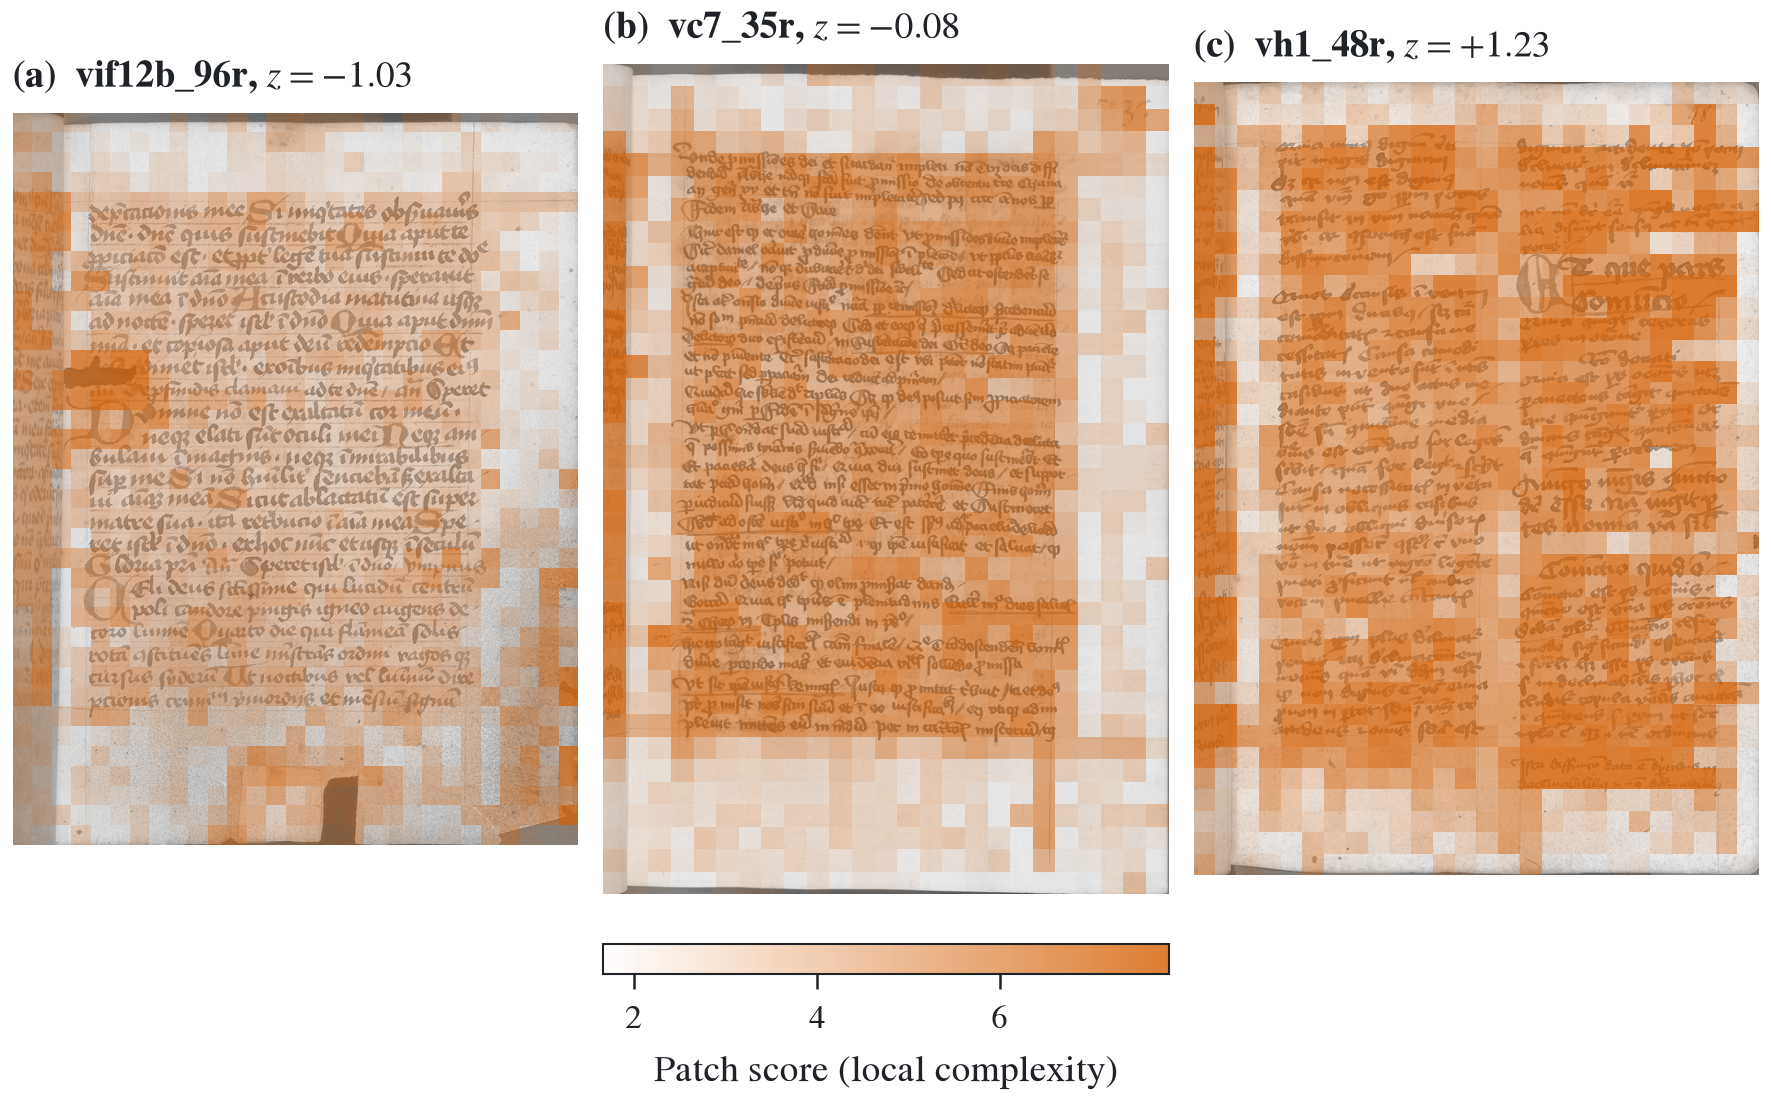
\includegraphics[width=15.00cm]{figures/local_complexity_maps.png}
  \caption{Local complexity maps: where the ViT head finds complexity on pages of low, middle and high predicted complexity, (a) vif12b\_96r ($z = -1.03$), (b) vc7\_35r ($z = -0.08$), (c) vh1\_48r ($z = +1.23$), scored above 17\%, 49\%, 87\% of the dataset's pages. Each 14-pixel patch of the folio crop, resized to 518 pixels on its long edge, is drawn with its score under the head trained on every judgment (on the patch tokens of DINOv2 ViT-S/14, block 12), in vermillion over the greyed page, on one colour scale for every page, from the 5th to the 95th percentile of the patch scores of all the dataset's pages (1.7 to 7.8), lower scores transparent and higher ones in full colour; the page's score is the mean of its patches'. $z$: the page's score, z-scored over the dataset's pages. Page images provided by Manuscriptorium (CC BY-NC 4.0).}
  \label{fig:local_complexity_maps}
\end{figure}
